\subsection{Night  Class Reference}
\label{class_night}\index{Night@{Night}}
version of the {\bf Reduced\-Image} {\rm (p.\,\pageref{class_reducedimage})}, quicker, but with more memory. 


{\tt \#include $<$night.h$>$}

Inheritance diagram for Night::\begin{figure}[H]
\begin{center}
\leavevmode
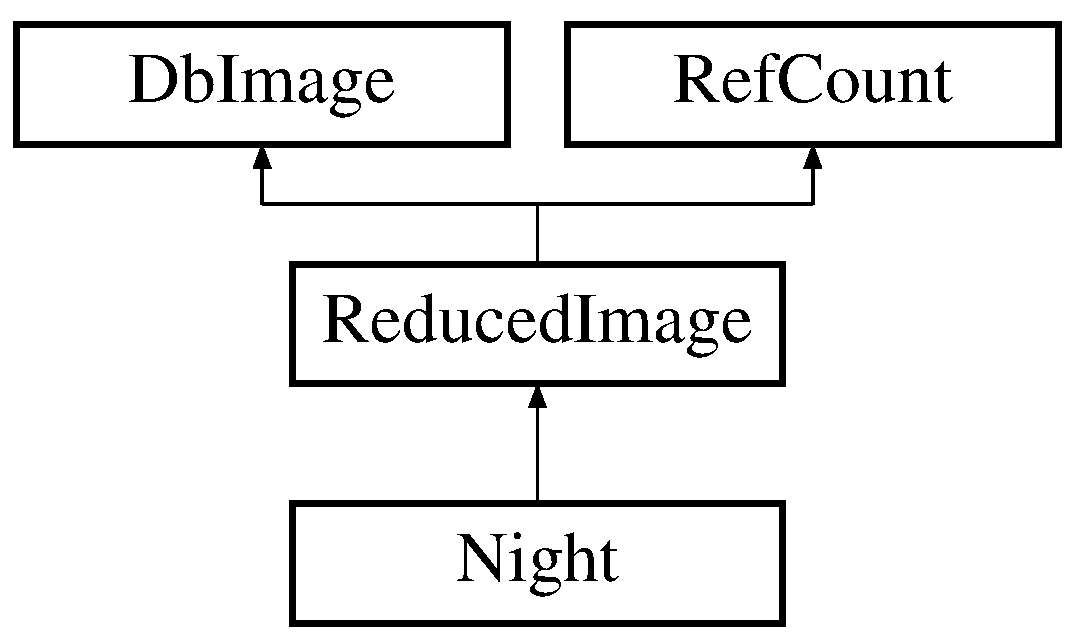
\includegraphics[height=3cm]{class_night}
\end{center}
\end{figure}
\subsubsection*{Public Methods}
\begin{CompactItemize}
\item 
\index{init@{init}!Night@{Night}}\index{Night@{Night}!init@{init}}
void {\bf init} ()\label{class_night_a0}

\begin{CompactList}\small\item\em Initialization of a night from its {\bf Reduced\-Image} {\rm (p.\,\pageref{class_reducedimage})}.\item\end{CompactList}\item 
\index{Night@{Night}!Night@{Night}}\index{Night@{Night}!Night@{Night}}
{\bf Night} (const string \&Name)\label{class_night_a1}

\item 
\index{Night@{Night}!Night@{Night}}\index{Night@{Night}!Night@{Night}}
{\bf Night} ()\label{class_night_a2}

\item 
\index{~Night@{$\sim$Night}!Night@{Night}}\index{Night@{Night}!~Night@{$\sim$Night}}
{\bf $\sim$Night} ()\label{class_night_a3}

\item 
\index{IsOK@{IsOK}!Night@{Night}}\index{Night@{Night}!IsOK@{Is\-OK}}
bool {\bf Is\-OK} () const\label{class_night_a4}

\begin{CompactList}\small\item\em returns true if the night verifies a bunch of criteria.\item\end{CompactList}\item 
\index{Clone@{Clone}!Night@{Night}}\index{Night@{Night}!Clone@{Clone}}
{\bf Reduced\-Image}$\ast$ {\bf Clone} () const\label{class_night_a5}

\begin{CompactList}\small\item\em copy constructor.\item\end{CompactList}\item 
\index{operator<@{operator$<$}!Night@{Night}}\index{Night@{Night}!operator<@{operator$<$}}
bool {\bf operator$<$} (const Night \&Right) const\label{class_night_a6}

\begin{CompactList}\small\item\em allows my\-Night1 $<$ my\-Night2 to sort in time.\item\end{CompactList}\item 
\index{dump@{dump}!Night@{Night}}\index{Night@{Night}!dump@{dump}}
void {\bf dump} (ostream \&Stream) const\label{class_night_a7}

\begin{CompactList}\small\item\em dumps basic info.\item\end{CompactList}\item 
\index{dump_header@{dump\_\-header}!Night@{Night}}\index{Night@{Night}!dump_header@{dump\_\-header}}
void {\bf dump\_\-header} (ostream \&Stream) const\label{class_night_a8}

\end{CompactItemize}
\subsubsection*{Public Attributes}
\begin{CompactItemize}
\item 
\index{saturation@{saturation}!Night@{Night}}\index{Night@{Night}!saturation@{saturation}}
double {\bf saturation}\label{class_night_m0}

\begin{CompactList}\small\item\em The saturation level.\item\end{CompactList}\item 
\index{photomRatio@{photomRatio}!Night@{Night}}\index{Night@{Night}!photomRatio@{photom\-Ratio}}
double {\bf photom\-Ratio}\label{class_night_m1}

\begin{CompactList}\small\item\em A photometric ratio with a given reference image.\item\end{CompactList}\item 
\index{kernelChi2@{kernelChi2}!Night@{Night}}\index{Night@{Night}!kernelChi2@{kernel\-Chi2}}
double {\bf kernel\-Chi2}\label{class_night_m2}

\begin{CompactList}\small\item\em A Chi2/Dof deriving from a kernel fitting procedure.\item\end{CompactList}\item 
\index{julianDate@{julianDate}!Night@{Night}}\index{Night@{Night}!julianDate@{julian\-Date}}
double {\bf julian\-Date}\label{class_night_m3}

\begin{CompactList}\small\item\em the julian date associated with the night.\item\end{CompactList}\item 
\index{exposure@{exposure}!Night@{Night}}\index{Night@{Night}!exposure@{exposure}}
double {\bf exposure}\label{class_night_m4}

\begin{CompactList}\small\item\em total exposure time for this night.\item\end{CompactList}\item 
\index{zeroPoint@{zeroPoint}!Night@{Night}}\index{Night@{Night}!zeroPoint@{zero\-Point}}
double {\bf zero\-Point}\label{class_night_m5}

\begin{CompactList}\small\item\em the zero point of the night.\item\end{CompactList}\item 
\index{seeing@{seeing}!Night@{Night}}\index{Night@{Night}!seeing@{seeing}}
double {\bf seeing}\label{class_night_m6}

\begin{CompactList}\small\item\em seeing (in pixel units) of the night.\item\end{CompactList}\item 
\index{sigmaX@{sigmaX}!Night@{Night}}\index{Night@{Night}!sigmaX@{sigma\-X}}
double {\bf sigma\-X}\label{class_night_m7}

\begin{CompactList}\small\item\em sigma (in pixel units) of the night PSF in x-direction.\item\end{CompactList}\item 
\index{sigmaY@{sigmaY}!Night@{Night}}\index{Night@{Night}!sigmaY@{sigma\-Y}}
double {\bf sigma\-Y}\label{class_night_m8}

\begin{CompactList}\small\item\em sigma (in pixel units) of the night PSF in y-direction.\item\end{CompactList}\item 
\index{thetaXY@{thetaXY}!Night@{Night}}\index{Night@{Night}!thetaXY@{theta\-XY}}
double {\bf theta\-XY}\label{class_night_m9}

\begin{CompactList}\small\item\em correlation angle of the night PSF.\item\end{CompactList}\item 
\index{skyLevel@{skyLevel}!Night@{Night}}\index{Night@{Night}!skyLevel@{sky\-Level}}
double {\bf sky\-Level}\label{class_night_m10}

\begin{CompactList}\small\item\em original sky background level of the night.\item\end{CompactList}\item 
\index{backLevel@{backLevel}!Night@{Night}}\index{Night@{Night}!backLevel@{back\-Level}}
double {\bf back\-Level}\label{class_night_m11}

\begin{CompactList}\small\item\em current background level of the image associated with the night.\item\end{CompactList}\item 
\index{sigmaSky@{sigmaSky}!Night@{Night}}\index{Night@{Night}!sigmaSky@{sigma\-Sky}}
double {\bf sigma\-Sky}\label{class_night_m12}

\begin{CompactList}\small\item\em sky RMS of the night sky background.\item\end{CompactList}\item 
\index{gain@{gain}!Night@{Night}}\index{Night@{Night}!gain@{gain}}
double {\bf gain}\label{class_night_m13}

\begin{CompactList}\small\item\em gain of the image (in e-/ADU).\item\end{CompactList}\item 
\index{flatError@{flatError}!Night@{Night}}\index{Night@{Night}!flatError@{flat\-Error}}
double {\bf flat\-Error}\label{class_night_m14}

\begin{CompactList}\small\item\em an estimate of the error in flatfielding (in \% of pixel intensity).\item\end{CompactList}\item 
\index{readoutNoise@{readoutNoise}!Night@{Night}}\index{Night@{Night}!readoutNoise@{readout\-Noise}}
double {\bf readout\-Noise}\label{class_night_m15}

\begin{CompactList}\small\item\em the readout noise in e-.\item\end{CompactList}\item 
\index{profileError@{profileError}!Night@{Night}}\index{Night@{Night}!profileError@{profile\-Error}}
double {\bf profile\-Error}\label{class_night_m16}

\begin{CompactList}\small\item\em the systematic error of the chosen PSF profile.\item\end{CompactList}\item 
\index{IsZeroRef@{IsZeroRef}!Night@{Night}}\index{Night@{Night}!IsZeroRef@{Is\-Zero\-Ref}}
bool {\bf Is\-Zero\-Ref}\label{class_night_m17}

\begin{CompactList}\small\item\em returns true if the night contribute as a zero point baseline for the lightcurve.\item\end{CompactList}\item 
\index{IsPhotometric@{IsPhotometric}!Night@{Night}}\index{Night@{Night}!IsPhotometric@{Is\-Photometric}}
bool {\bf Is\-Photometric}\label{class_night_m18}

\begin{CompactList}\small\item\em returns true if the night is photometric.\item\end{CompactList}\end{CompactItemize}
\subsubsection*{Friends}
\begin{CompactItemize}
\item 
class {\bf operator$<$$<$}
\end{CompactItemize}


\subsubsection{Detailed Description}
version of the {\bf Reduced\-Image} {\rm (p.\,\pageref{class_reducedimage})}, quicker, but with more memory.



The documentation for this class was generated from the following file:\begin{CompactItemize}
\item 
{\bf night.h}\end{CompactItemize}
